\documentclass{ReportTemplate}
\usepackage{titlesec}
\title{Projet Interdisciplinaire}
\author{Macherel Rémy}
\date{\today}
\subtitle{Soutien aux personnes atteintes de cancer}
\subsubtitle{}
\location{Fribourg,}
\contact{remy.macherel@master.hes-so.ch}
\version{1.0}
\titlespacing*{\chapter}{0pt}{-60pt}{20pt}

\begin{document}
\maketitlepage
\newpage
\maketableofcontent
\medskip

\titleformat{\chapter}[display]
    {\Huge\bfseries}
    {}
    {0pt}
    {\thechapter.\ }

\chapter{Introduction}
Dans le cadre du projet Interdisciplinaire du master mse semestre de Printemps
2022, nous avons décidé de réaliser un projet de recherche sur les personnes
atteintes de cancer et plus particulièrement sur le développement d'un outil
permettant de simplifier la situation de ces personnes d'un point de vue de
l'accès à l'information afin de leur fournir des informations claires et
correctes afin de diminuer leur tendance au stress. Ce projet sera guidé par le
thème du \textit{Design Thinking} et ses différentes phases seront appliquées.


\chapter{Phase 1, Empathy}
\section{Discussion avec des experts}
Dans le cadre de la première phase du \textit{Design Thinking} (phase
d'empathie), nous avons tout d'abord rencontré Mme. Chopard afin d'avoir des
informations de la part d'une experte sur le sujet et sur les différentes études
déjà menées à ce sujet.
Nous avons rencontré en date du 24.03.2022 Mme. Saba Chopard dans le cadre d'une
séance de présentation et de discussion autour du thème du cancer et plus
particulièrement du stress des patients ainsi que l'accès à l'information de
ceux-ci. Nous avions pour ceci préparé quelques questions à poser et nous avons
rassemblé ces questions ainsi que les réponses de Mme. Chopard à certaines
d'entre elles dans un document annexe (voir document Discussion\_24032022 dans
annexes).
\section{Prise de contact avec patiente et interview}
Durant cette phase, nous avons également pris contact avec une patiente
actuellement guérie du cancer afin de connaitre son point de vue et d'avoir un
ressenti sur ses expériences afin de pouvoir continuer nos
recherches.%TODO: Add interview questions + answers 
\newpage
\section{Empathy Map}
L'interview ainsi que la discussion avec l'experte nous ont permis de dresser
\textit{Empathy Map} qui est un outil de réflexion sur les différents aspects
émotionnels des patients.
\begin{figure}[H]
    \centering
    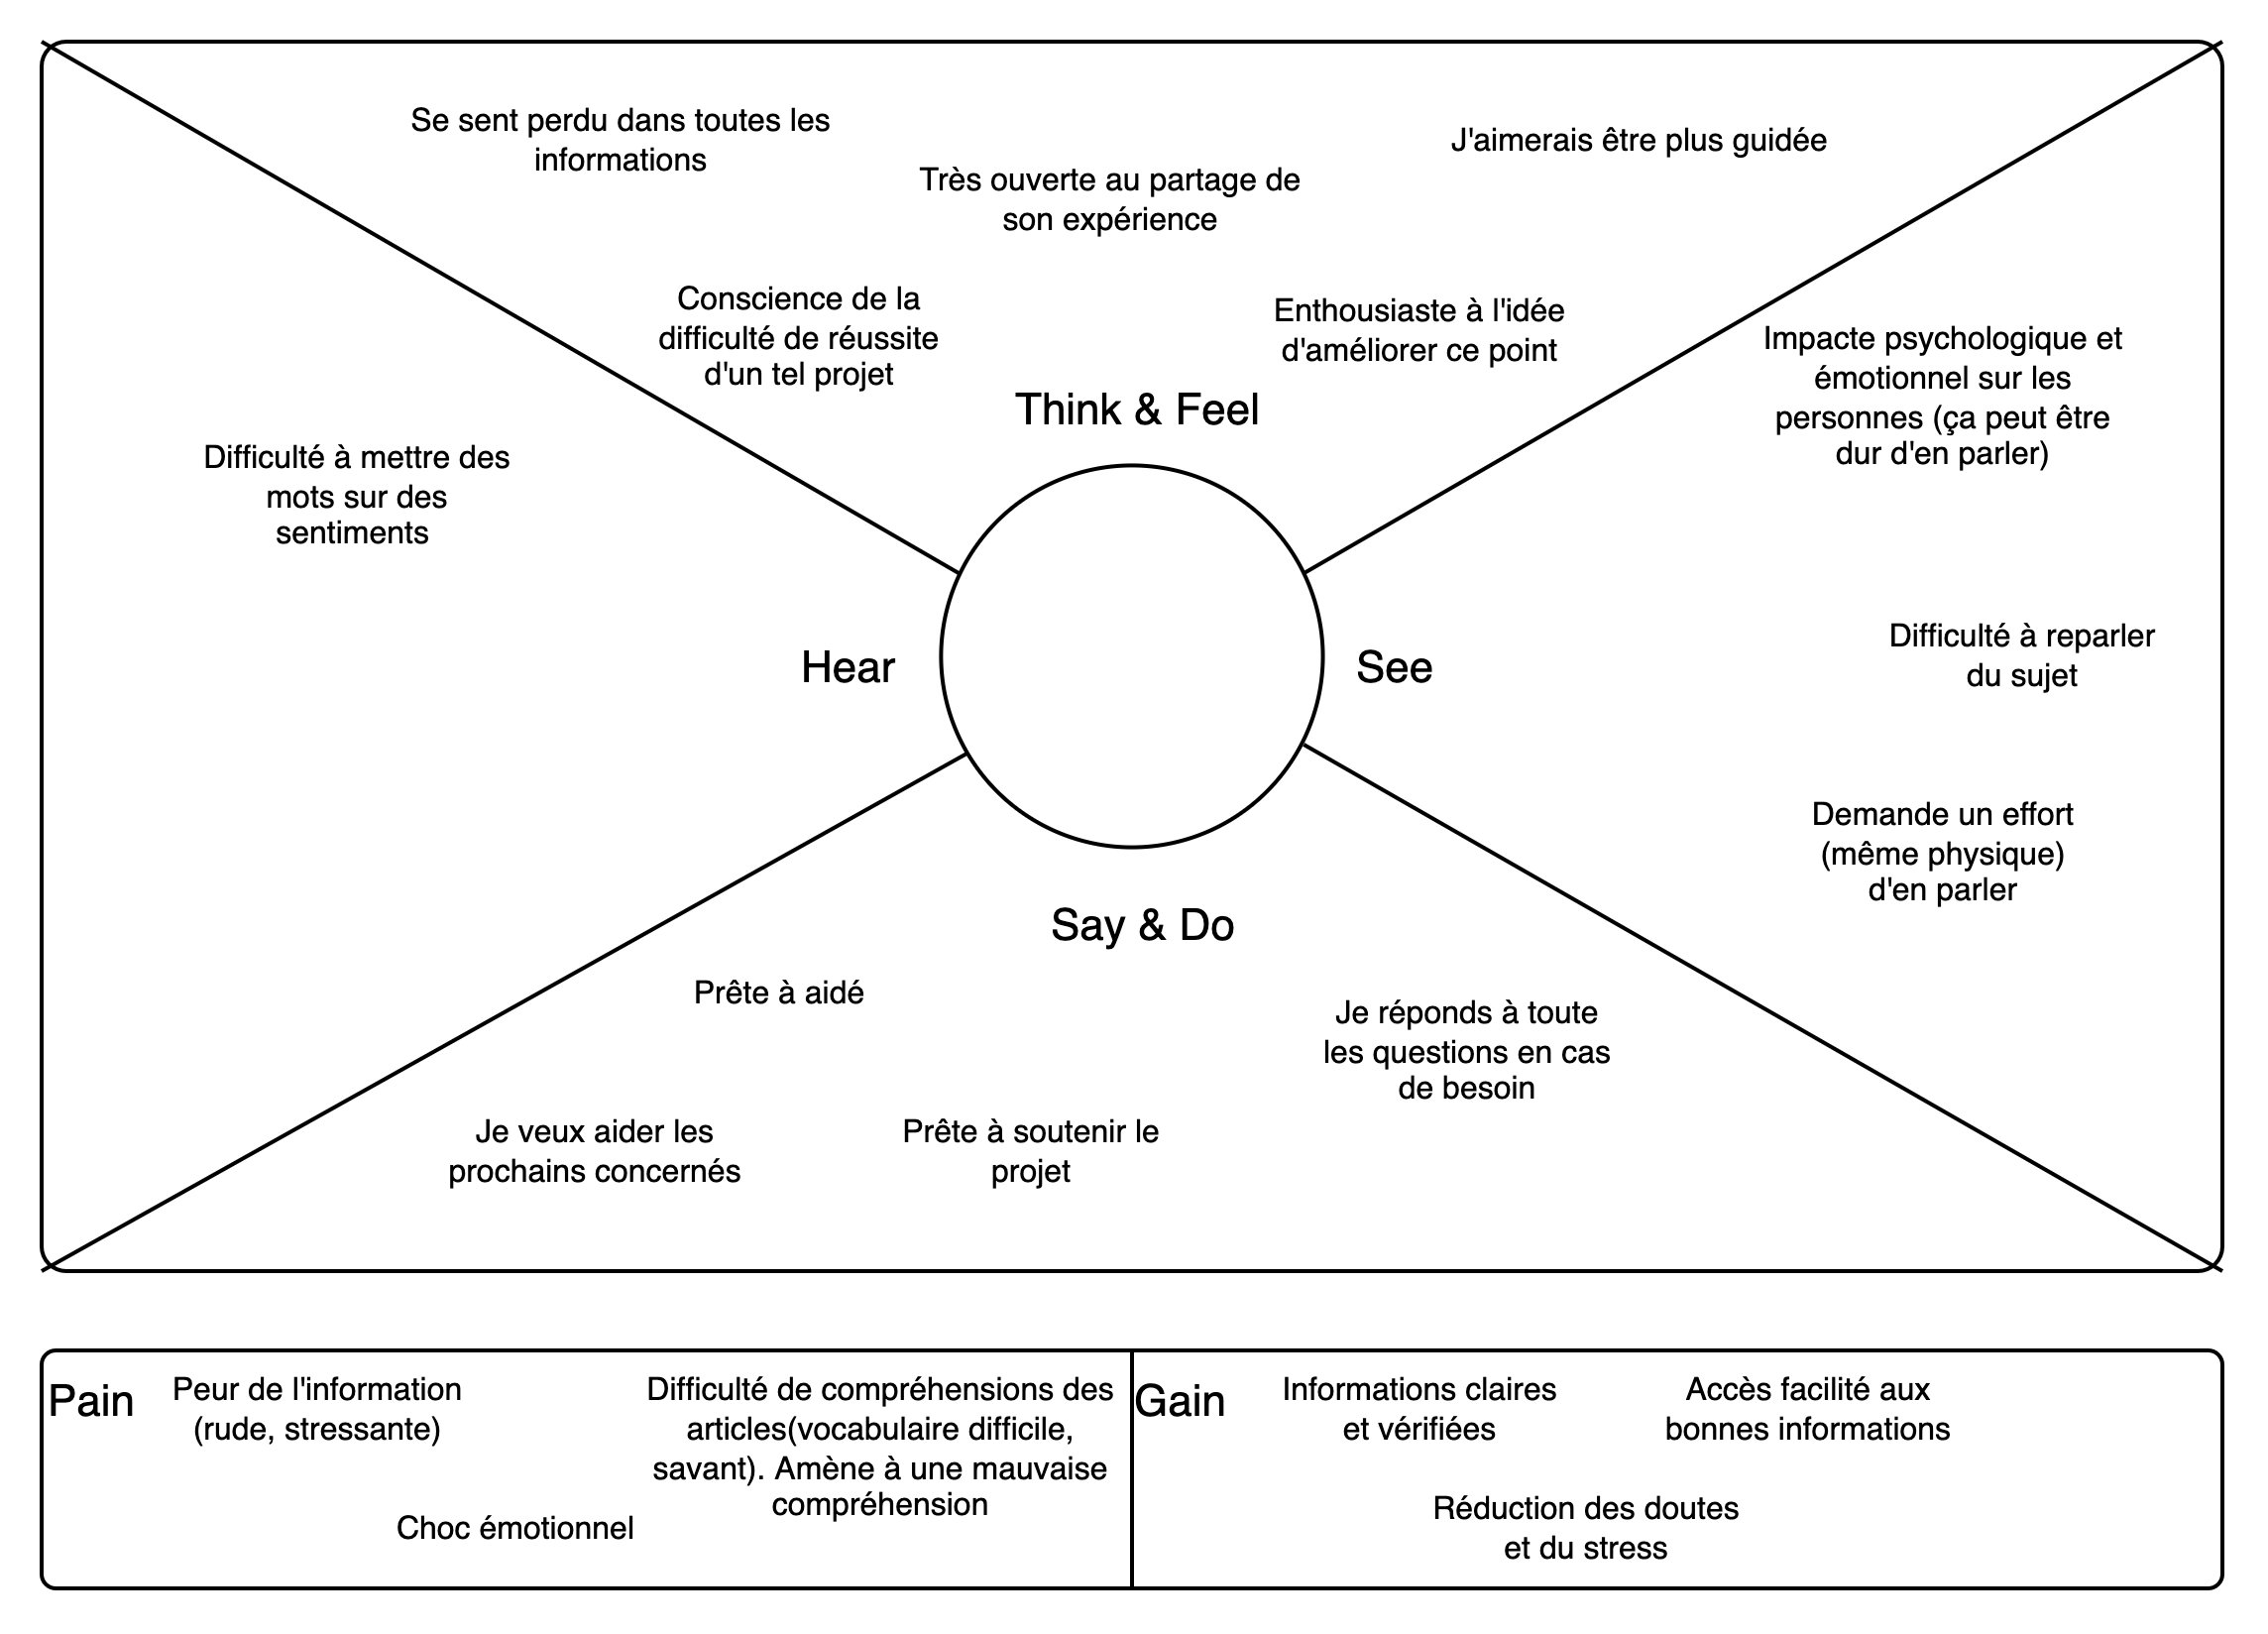
\includegraphics[width=\textwidth]{imageSources/EmpathyMap.png}
    \caption{Empathy Map}
    \label{fig:EmpathyMap}
\end{figure}
\chapter{Phase 2, Define}
Dans cette phase, nous utilisons les informations récoltées lors de la séance
avec Mme. Chopard ainsi que les résultats de l'interview avec la patiente afin
de cibler au mieux le sujet à traiter ainsi que de pouvoir se concentrer sur une
problématique claire.
\section{Mind Map brainstorming}
Nous avons ensuite réalisé un mind-map avec les différentes informations reçues
lors de cette rencontre afin de sythétiser celles-ci.
\begin{figure}[H]
    \centering
    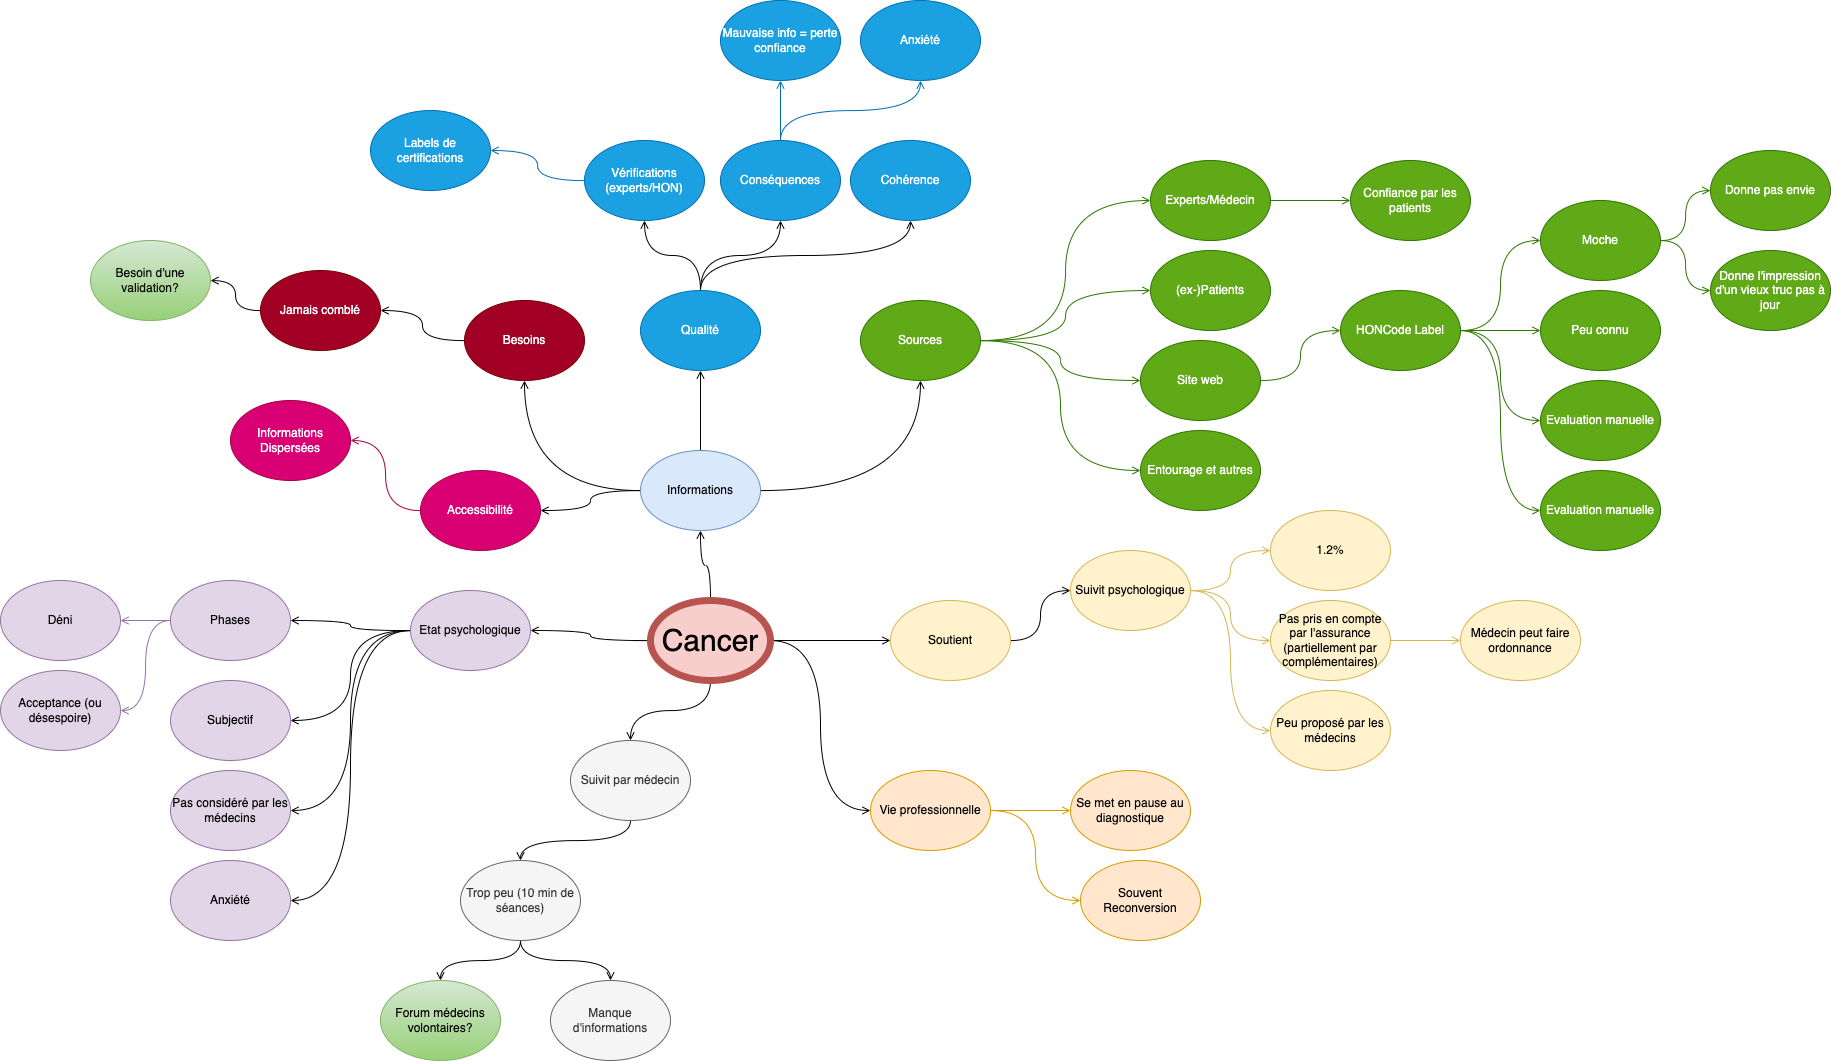
\includegraphics[width=\textwidth]{imageSources/PI-Expert-MM.png}
    \caption{Mind Map (see also in annexes)}
    \label{fig:MindMap}
\end{figure}
\section{Personas}
Nous avons déclaré deux personas pouvant correspondre aux potentiels sujets de
notre projet. Ceux-ci furent créés afin de combler les sujets potentiels à notre projet.
\begin{figure}[H]
    \centering
    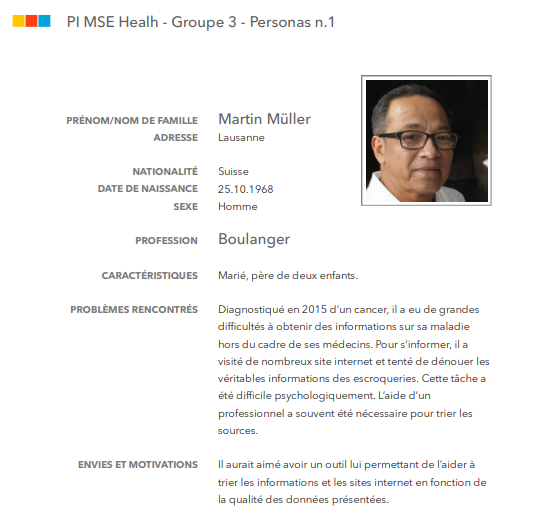
\includegraphics[width=\textwidth]{imageSources/Persona_1.png}
    \caption{Persona numéro 1}
    \label{fig:Persona1}
\end{figure}
\begin{figure}[H]
    \centering
    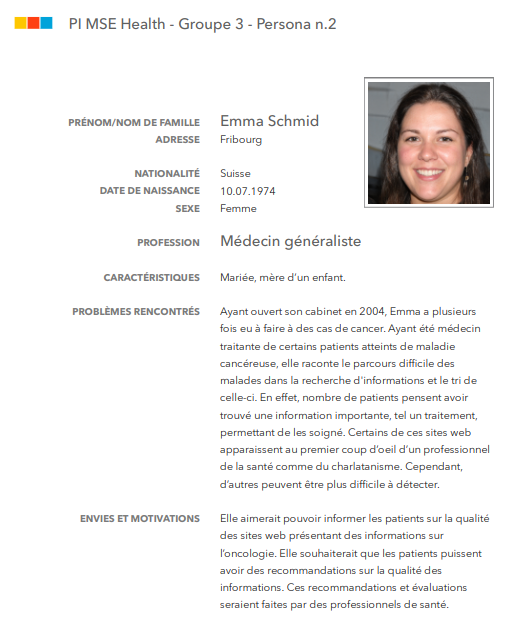
\includegraphics[width=\textwidth]{imageSources/Persona_2.png}
    \caption{Persona numéro 2}
    \label{fig:Persona2}
\end{figure}

\chapter{Phase 3, Ideate}
Lors de la phase 3, nous avons pris les résultats de l'interview ainsi que les
informations trouvées par nos soins afin de regrouper toutes les idées
potentielles de produits ou services pouvant assouvir le besoin d'information
des patients tout en assurant la véracité de ces informations. Nous avons
également mis l'accent sur la qualité de l'information mais aussi la facilité
d'accès à celle-ci. La première phase de réfléxion est disponible sur la figure
suivante :
\begin{figure}[H]
    \centering
    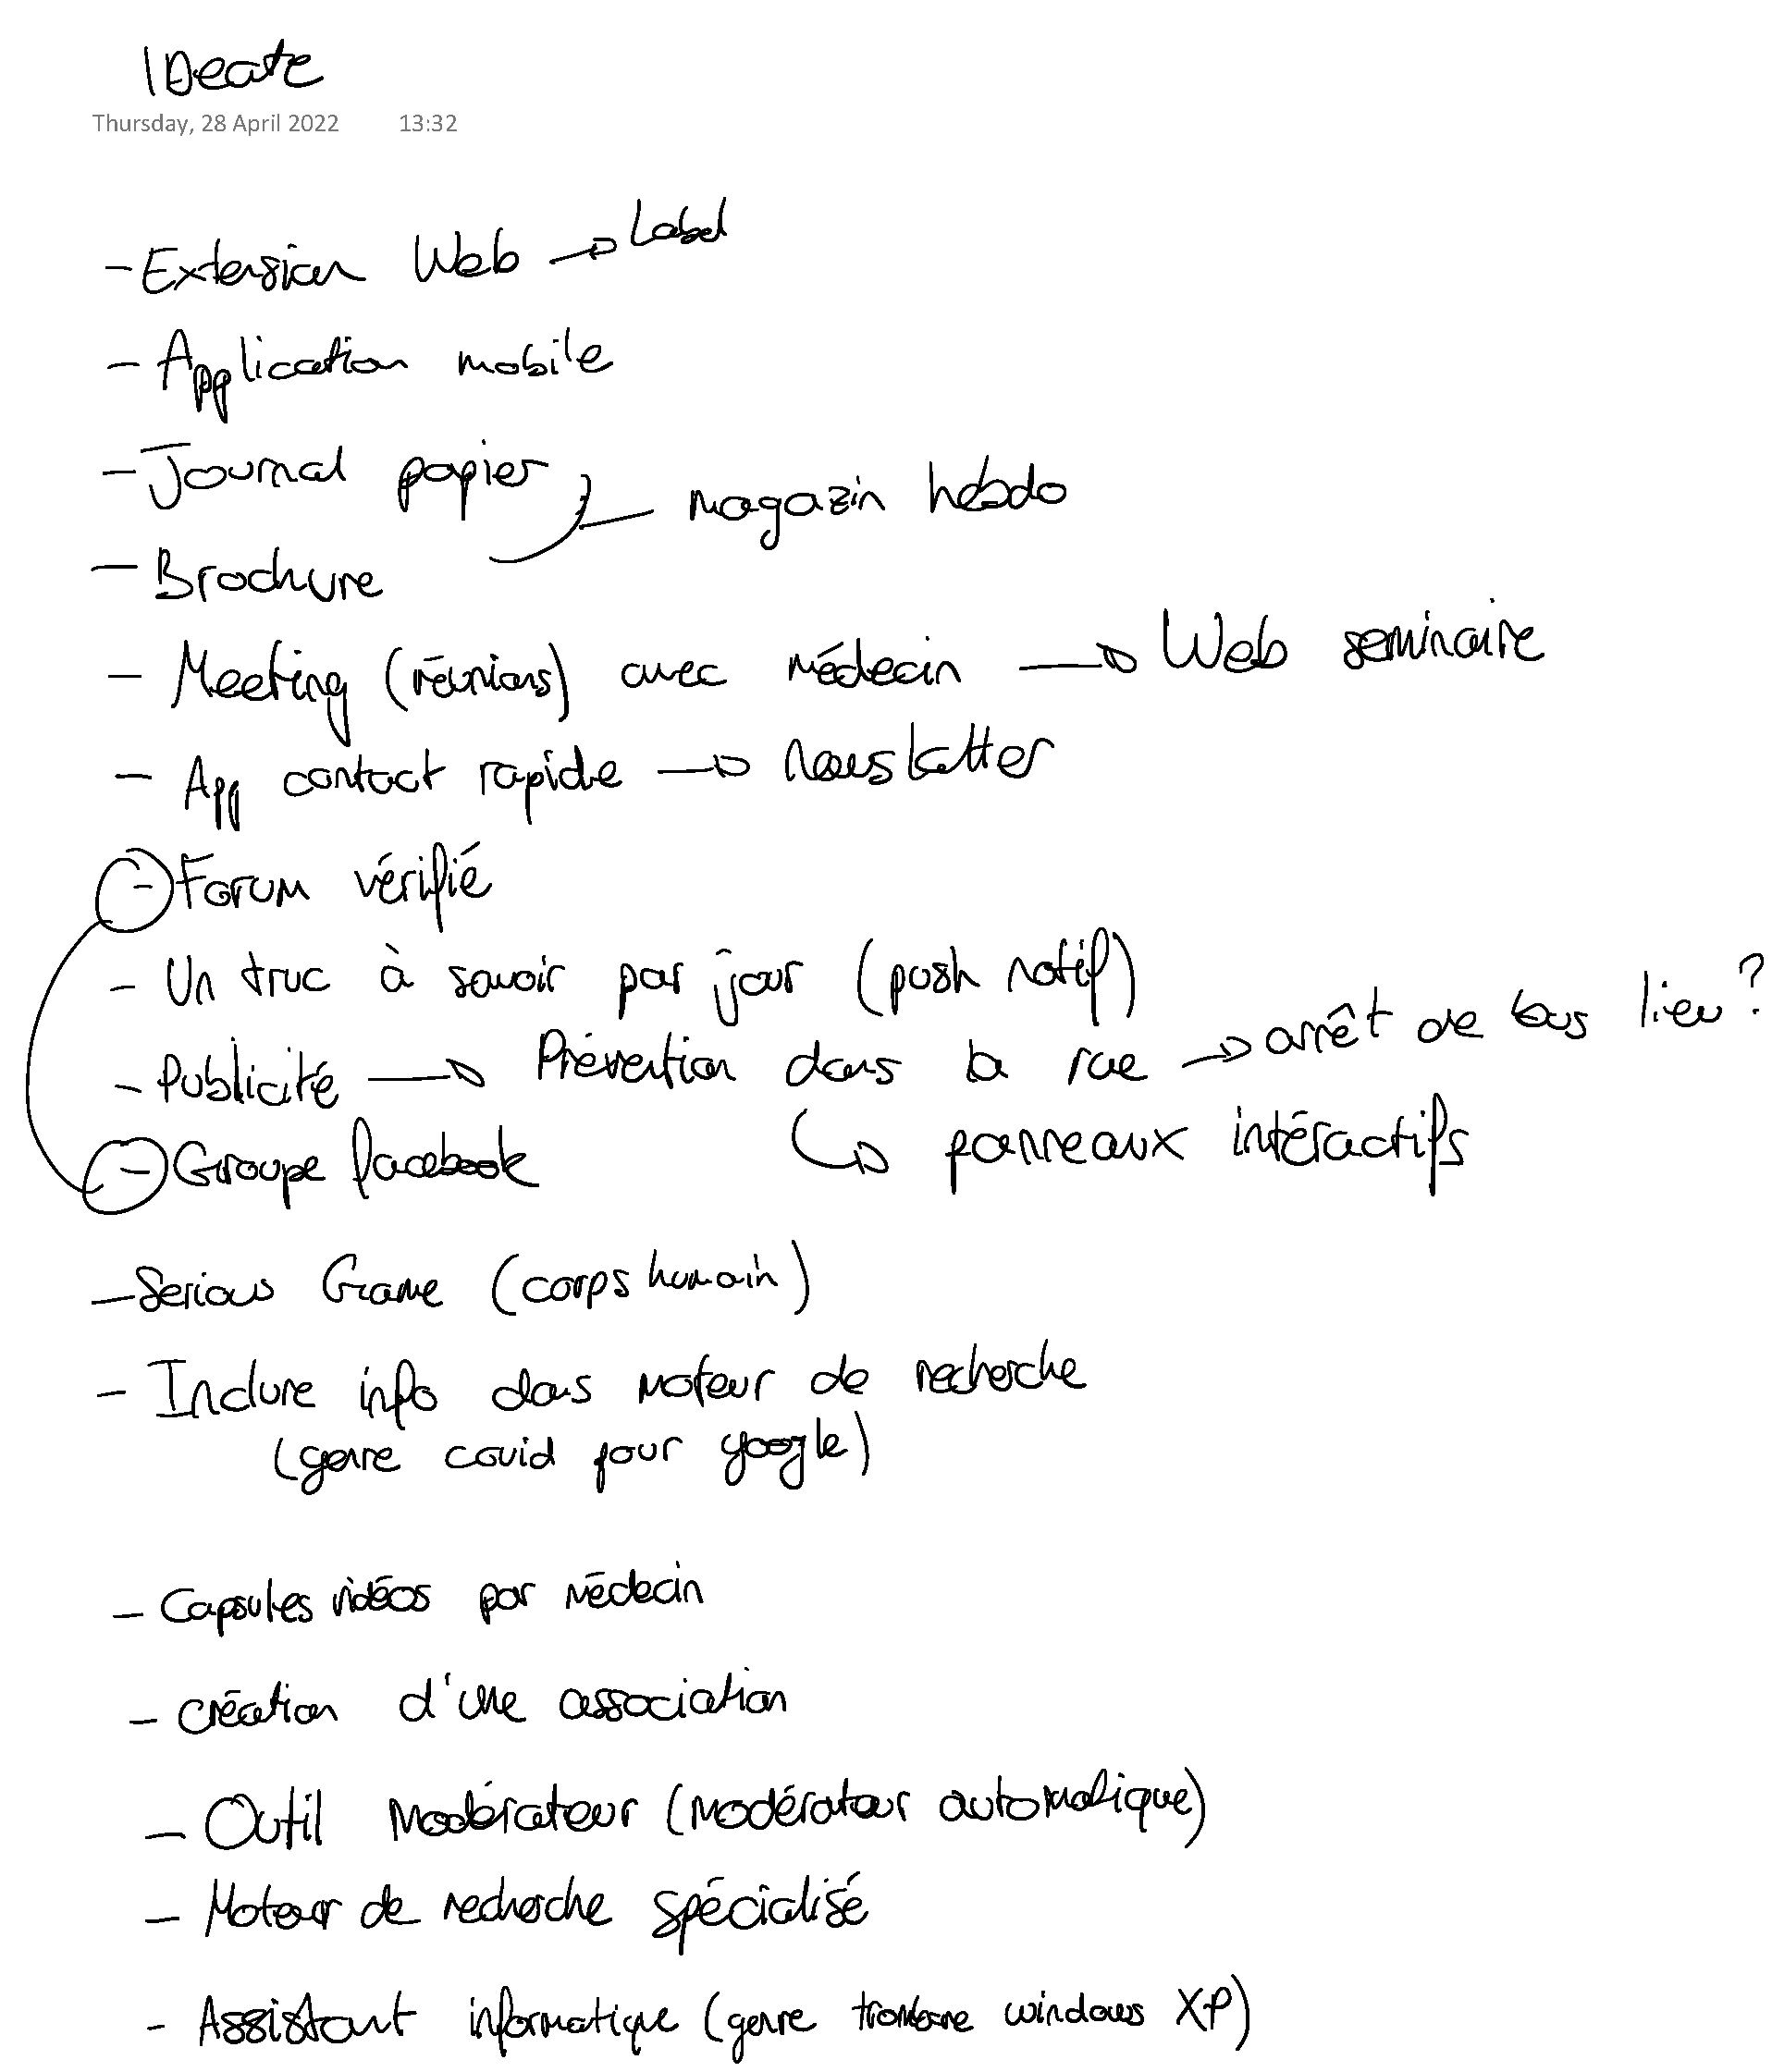
\includegraphics[width=\textwidth]{Annexes/Ideate_1.pdf}
    \caption{Phase d'idéation brouillon}
    \label{fig:Ideate1_brouillon}
\end{figure}
Nous avons ensuite regroupé et classé ces idées de la manière suivante :
\begin{figure}[H]
    \centering
    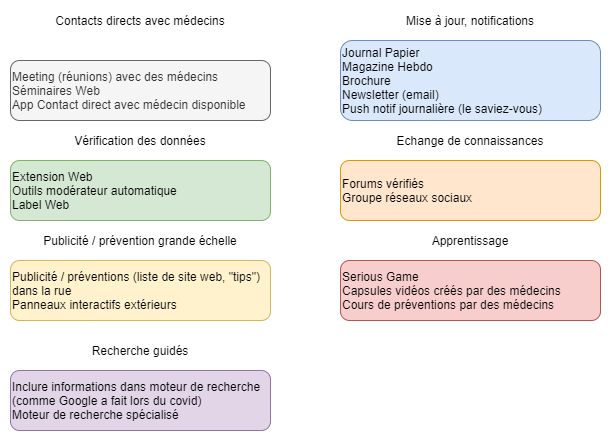
\includegraphics[width=\textwidth]{imageSources/Ideate_1.png}
    \caption{Phase d'idéation}
    \label{fig:Ideate1}
\end{figure}
\newpage
Durant cette phase nous avons également rapidement établi un visuel de ce que
pourrait être l'extension web:
\begin{figure}[H]
    \centering
    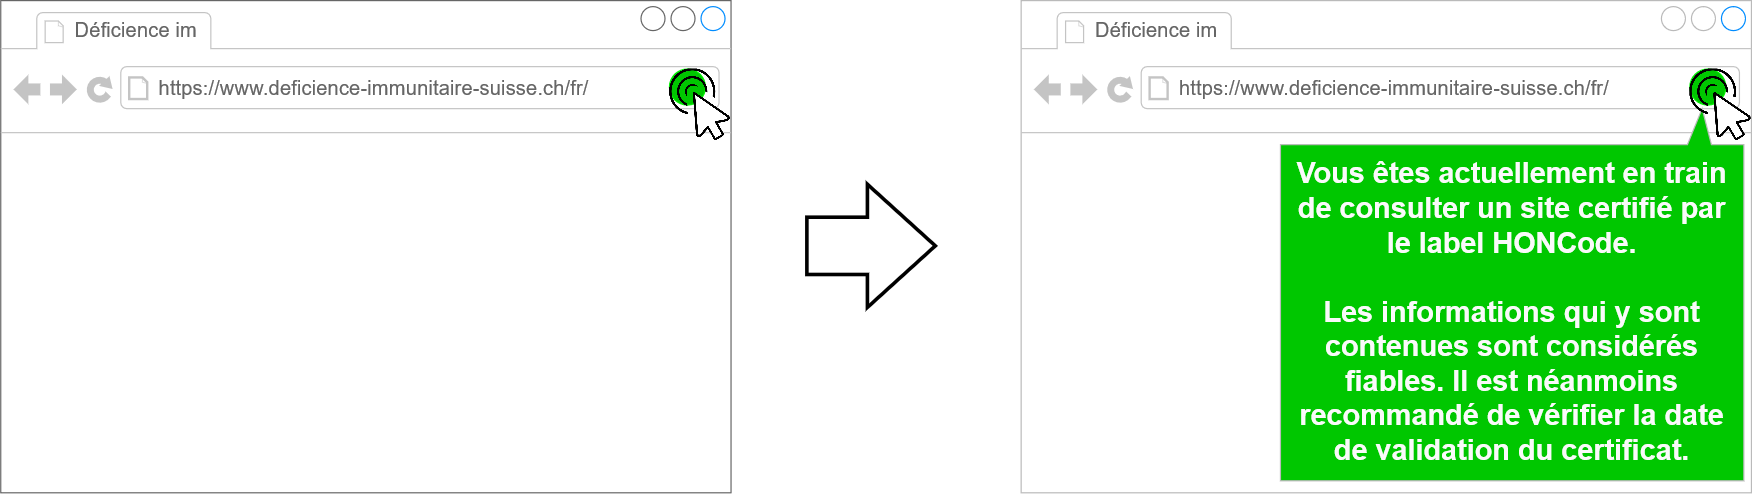
\includegraphics[width=\textwidth]{imageSources/Exemple_Extension_1.png}
    \caption{Site certifié HonCode}
    \label{fig:ExempleExt1}
\end{figure}
\begin{figure}[H]
    \centering
    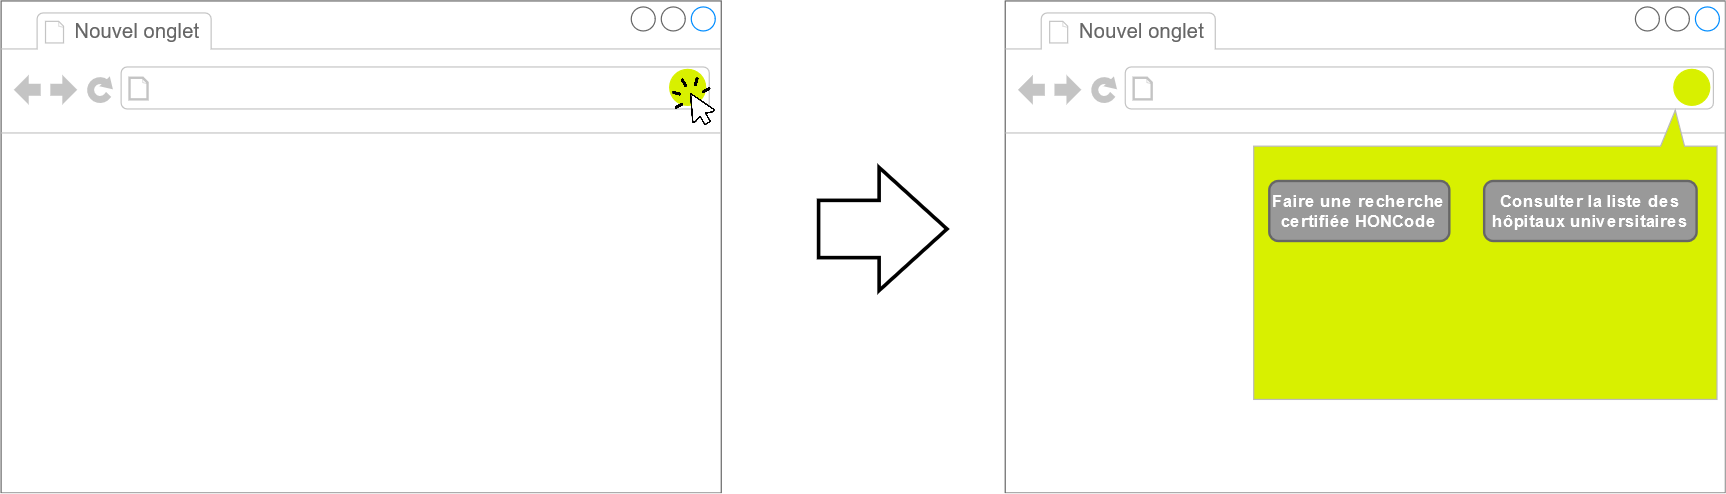
\includegraphics[width=\textwidth]{imageSources/Exemple_Extension_2.png}
    \caption{Proposition de recherche}
    \label{fig:ExempleExt2}
\end{figure}
\begin{figure}[H]
    \centering
    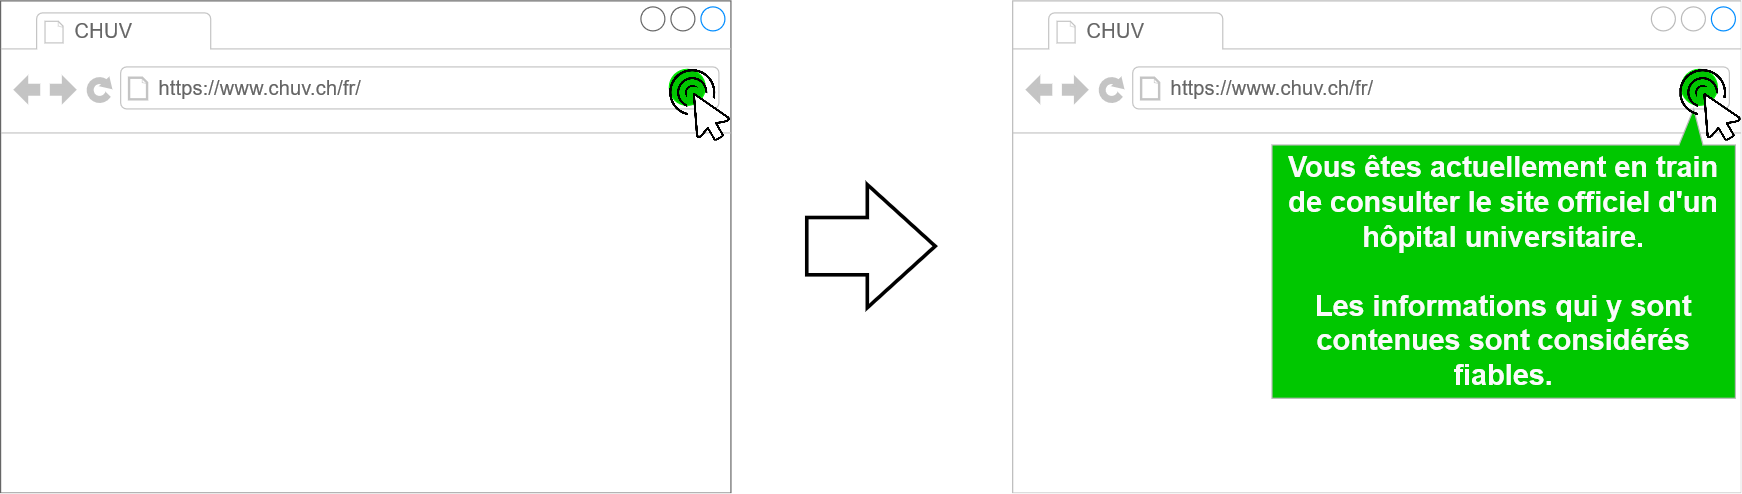
\includegraphics[width=\textwidth]{imageSources/Exemple_Extension_3.png}
    \caption{Site universitaire ou confirmé}
    \label{fig:ExempleExt3}
\end{figure}
\begin{figure}[H]
    \centering
    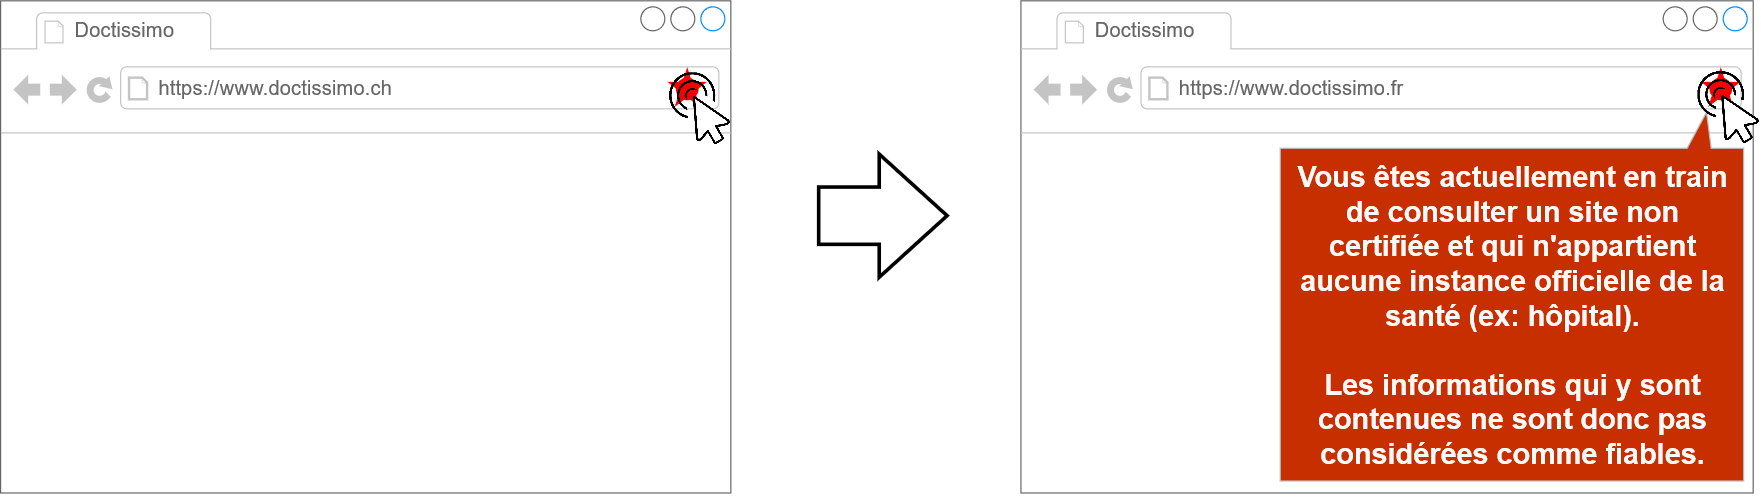
\includegraphics[width=\textwidth]{imageSources/Exemple_Extension_4.png}
    \caption{Site non certifié HonCode et pas universitaire ou confirmé}
    \label{fig:ExempleExt4}
\end{figure}

Nous avons ensuite décidé de recontacter les clients (et patients) afin qu'ils
puissent évaluer ces idées et nous donner un feedback afin de pouvoir concevoir
le projet le plus proche de leurs besoins possible.

\end{document}


